
\chapter{Estudio del Arte}

\setlength{\parindent}{5ex}En este capitulo se hablara de porque se han elegido las tecnologías que se van a utilizar en el proyecto asi como mostrar algunas de las opciones adicionales que se podrían haber utilizado. 

\section{¿Porque Arduino?}

Arduino es una plataforma Hardware Open Source lo que implica que todo el sistema esta disponible a los usuarios y esto ayudara al proceso de montaje ya que una gran parte de personas (la comunidad de Arduino) trabajan de manera desinteresada en el desarrollo de librerías y aplicaciones para esta plataforma. 
\setlength{\parindent}{0ex}

Sin embargo Arduino dispone de numerosas versiones por lo que dentro de las mas famosas que hay he decidido analizar cual de los que hay me ofrece mas garantías a la hora de realizar el proyecto por lo que en principio me decantare por el consumo de las microcontroladora, puertos y conexiones disponibles y disponibilidad.

En primer lugar he realizado un estudio del consumo de las placas disponibles para poder realizar este proyecto, 

\begin{center}
	\begin{tabular}{c c c } 
		\hline
		\textbf{Board} & \textbf{Consumo(W/h)} & \textbf{Consumo(mA/h)} \\ [0.3ex] 
		\specialrule{.08em}{1em}{0em}
		Arduino UNO & 0.23 & 46  \\ 
		Arduino DUE & 0.375 & 75  \\
		Arduino MEGA & 0.465 & 93  \\
		Arduino Nano & 0.075 & 15  \\
		Raspberry Pi & 1.77 & 353  \\ [1ex] 
		\hline
	\end{tabular}
	\captionof{table}{Consumo de los diferentes dispositivos} \label{tab:table1} 
\end{center}

En este caso nos interesaría el elegir el dispositivo que menor consumo tenga pero también he tenido que mirar que funcionalidad pueden aportar cada placa, cabe destacar que la Raspberry Pi no es una microcontroladora, si no un ordenador de placa reducida, pero ofrece una funcionalidad que podría mejorar las prestaciones de este proyecto, hablando de seguridad y comunicación, pero sin embargo después de las pruebas de consumo comparando con el Arduino que mas consume, en este caso el MEGA, consume en mA un 379\% mas ya que necesita mantener un sistema operativo que aunque sigue siendo un consumo muy bajo para ser un ordenador, es muy elevado para este proyecto así que en este punto descartamos la Raspberry Pi.

Otro punto a tener en cuenta son las capacidades de conexión que tienen las microcontroladoras, ya que para poder conectarlo todo voy a necesitar 3 entradas analógicas, una  entrada digital, 2 entradas para el rx y tx del puerto serie y compatibilidad con la Shield ethernet de Arduino.

El Arduino UNO es una muy buena opción ya que tiene todo esto y es de un consumo reducido aun así, la comunicación serial va por software ya que hay que implementar una librería especial para poder realzar un puerto serie para comunicarse con el GPS, ademas habría que diseñar un circuito por los problemas en los voltajes de las lecturas digitales ya que algunos componentes devuelven 3.3V y Arduino los detecta a 5V, que bien que no daría problemas pero podría dar lugar a valores anómalos en determinadas ocasiones.

El Arduino MEGA es la mejor opción disponible sin embargo ajustando con el material disponible, he de elegir el Arduino DUE ya que tiene un consumo mas reducido.

Estas son las características del Arduino DUE:

\begin{itemize}
\item \textbf{Microcontrolador}: AT91SAM3X8E
\item \textbf{Velocidad de reloj:} 84 MHz
\item \underline{\textbf{Tensión de trabajo:} 3.3V}
\item \underline{\textbf{Pines de entradas digitales:} 54}
\item \underline{\textbf{Pines de entradas analógicas: }12}
\item \underline{\textbf{Memoria Flash:} 512 KB}
\end{itemize}

He subrayado los valores que son importantes ya que en el estudio del montaje en el Arduino UNO tenia problemas con la memoria del programa ya que la memoria Flash quedaba casi completa utilizando la librería que implementaba un serial en cualquier pin digital,  imposibilitando la capacidad de poder implementar mejoras en la aplicación.

\section{Presupuesto}

En esta parte del proyecto se va a realizar un estudio de lo que puede llegar a costar la creación, el montaje y el mantenimiento de la aplicación, todo ello al precio actual del año 2016.

Em primer lugar se expondrá el coste de que costaría aproximadamente cada nodo de la aplicación:

\begin{itemize}
	\item \textbf{Arduino DUE:} 36\euro 
	\item \textbf{Shield de Ethernet:} 26\euro 
	\item \textbf{Neo6Mv2:} 13,50\euro 
	\item \textbf{Sensor de Gas MQ-7:} 8\euro 
	\item \textbf{Sensor de Temperatura y Humedad DHT11:} 3\euro 
	\item \textbf{Sensor de Sonido:} 0,50\euro 
	\item \textbf{Sensor de Luz:} 1\euro 
\end{itemize}

Todo esto nos da un coste de \textbf{88 \euro} por nodo de sensores aproximadamente.

Se podrían utilizar materiales mas baratos con el fin de reducir los costes aun mas pero no seria aconsejable pues del proyecto interesa que este activo el mayor tiempo posible. También se pueden modificar los elementos del mismo, nombrados en la parte donde se realizaba el estudio del consumo de energía de cada controladora (\textbf{Tabla \ref{tab:table1}}) realizando las modificaciones necesarias para que este pueda funcionar.

También se ha incluido el coste de lo que costaría añadir el servidor de la aplicación, en este caso he puesto componentes genéricos:

\begin{itemize}
	\item \textbf{Servidor:} 600\euro 
	\item \textbf{Router:} 30\euro 
	\item \textbf{Cableado:} 12\euro 
\end{itemize}

Todo esto nos da un coste de \textbf{642 \euro} por servidor aproximadamente, pero, como se ha explicado antes, todo esto se puede reducir con material ya disponible, porque, "quien no tiene un ordenador hoy día?".

Y por ultimo el mantenimiento de lo que seria todo el montaje, ya es difícil hablar de un mantenimiento pues la aplicación pues aumentaría con cada nodo añadido, la ampliación del servidor en caso de haber demasiadas peticiones, el modo de alimentar los nodos que podría ser por microUSB, POE o baterías, diferentes Controladoras, todo esto nos daría un resultado muy variable, así que es muy complicado cuanto costaría mantener la aplicación.

\section{Gestión del proyecto}

Para este proyecto se va a gestionar el proyecto utilizando una aplicación Web llamada \textit{Bitbucket}:

\textit{Bitbucket es un servicio de alojamiento basado en web, para los proyectos que utilizan el sistema de control de revisiones Mercurial y Git.}\cite{bitbucket}.

En esta aplicación se irán subiendo todos los cambios que se realicen en este proyecto ya que ofrece una gestión bastante sencilla de los proyectos y las versiones de cada una, ademas cuenta con una aplicación llamada \textit{sourceTree} que permite conectar con una cuenta de \textit{Bitbucket} y permitirá realizar las subidas de ficheros desde el mismo sistema operativo sin tener que acceder desde el navegador y ademas gestionar de una manera sencilla todas las versiones del proyecto.

\begin{figure}[!h]
	\centering
	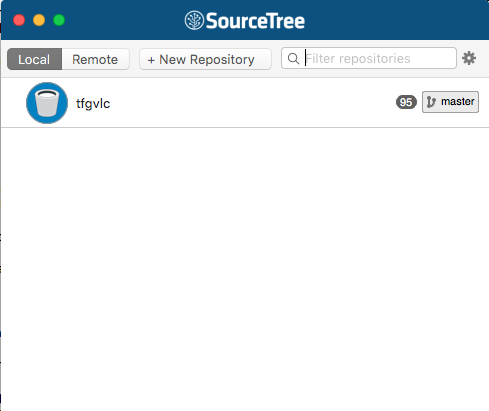
\includegraphics[width=0.3\linewidth]{figuras/stree}
	\caption{Gestion de proyectos con \textit{SourceTree}}
	\label{fig:stree}
\end{figure}
